\appendix
\addtocontents{toc}{\protect\setcounter{tocdepth}{-5}}
\chapter{User manual}

Due to this application being entered as a practical demonstration running on a Raspberry Pi board, this manual
provides the information necessary in the end to end preparation of the demo. This will help in correctly
setting up the Raspberry Pi, building and installing the application, and understanding the features
provided by the application.

\section{Raspberry Pi Setup}

\begin{figure}[H]
	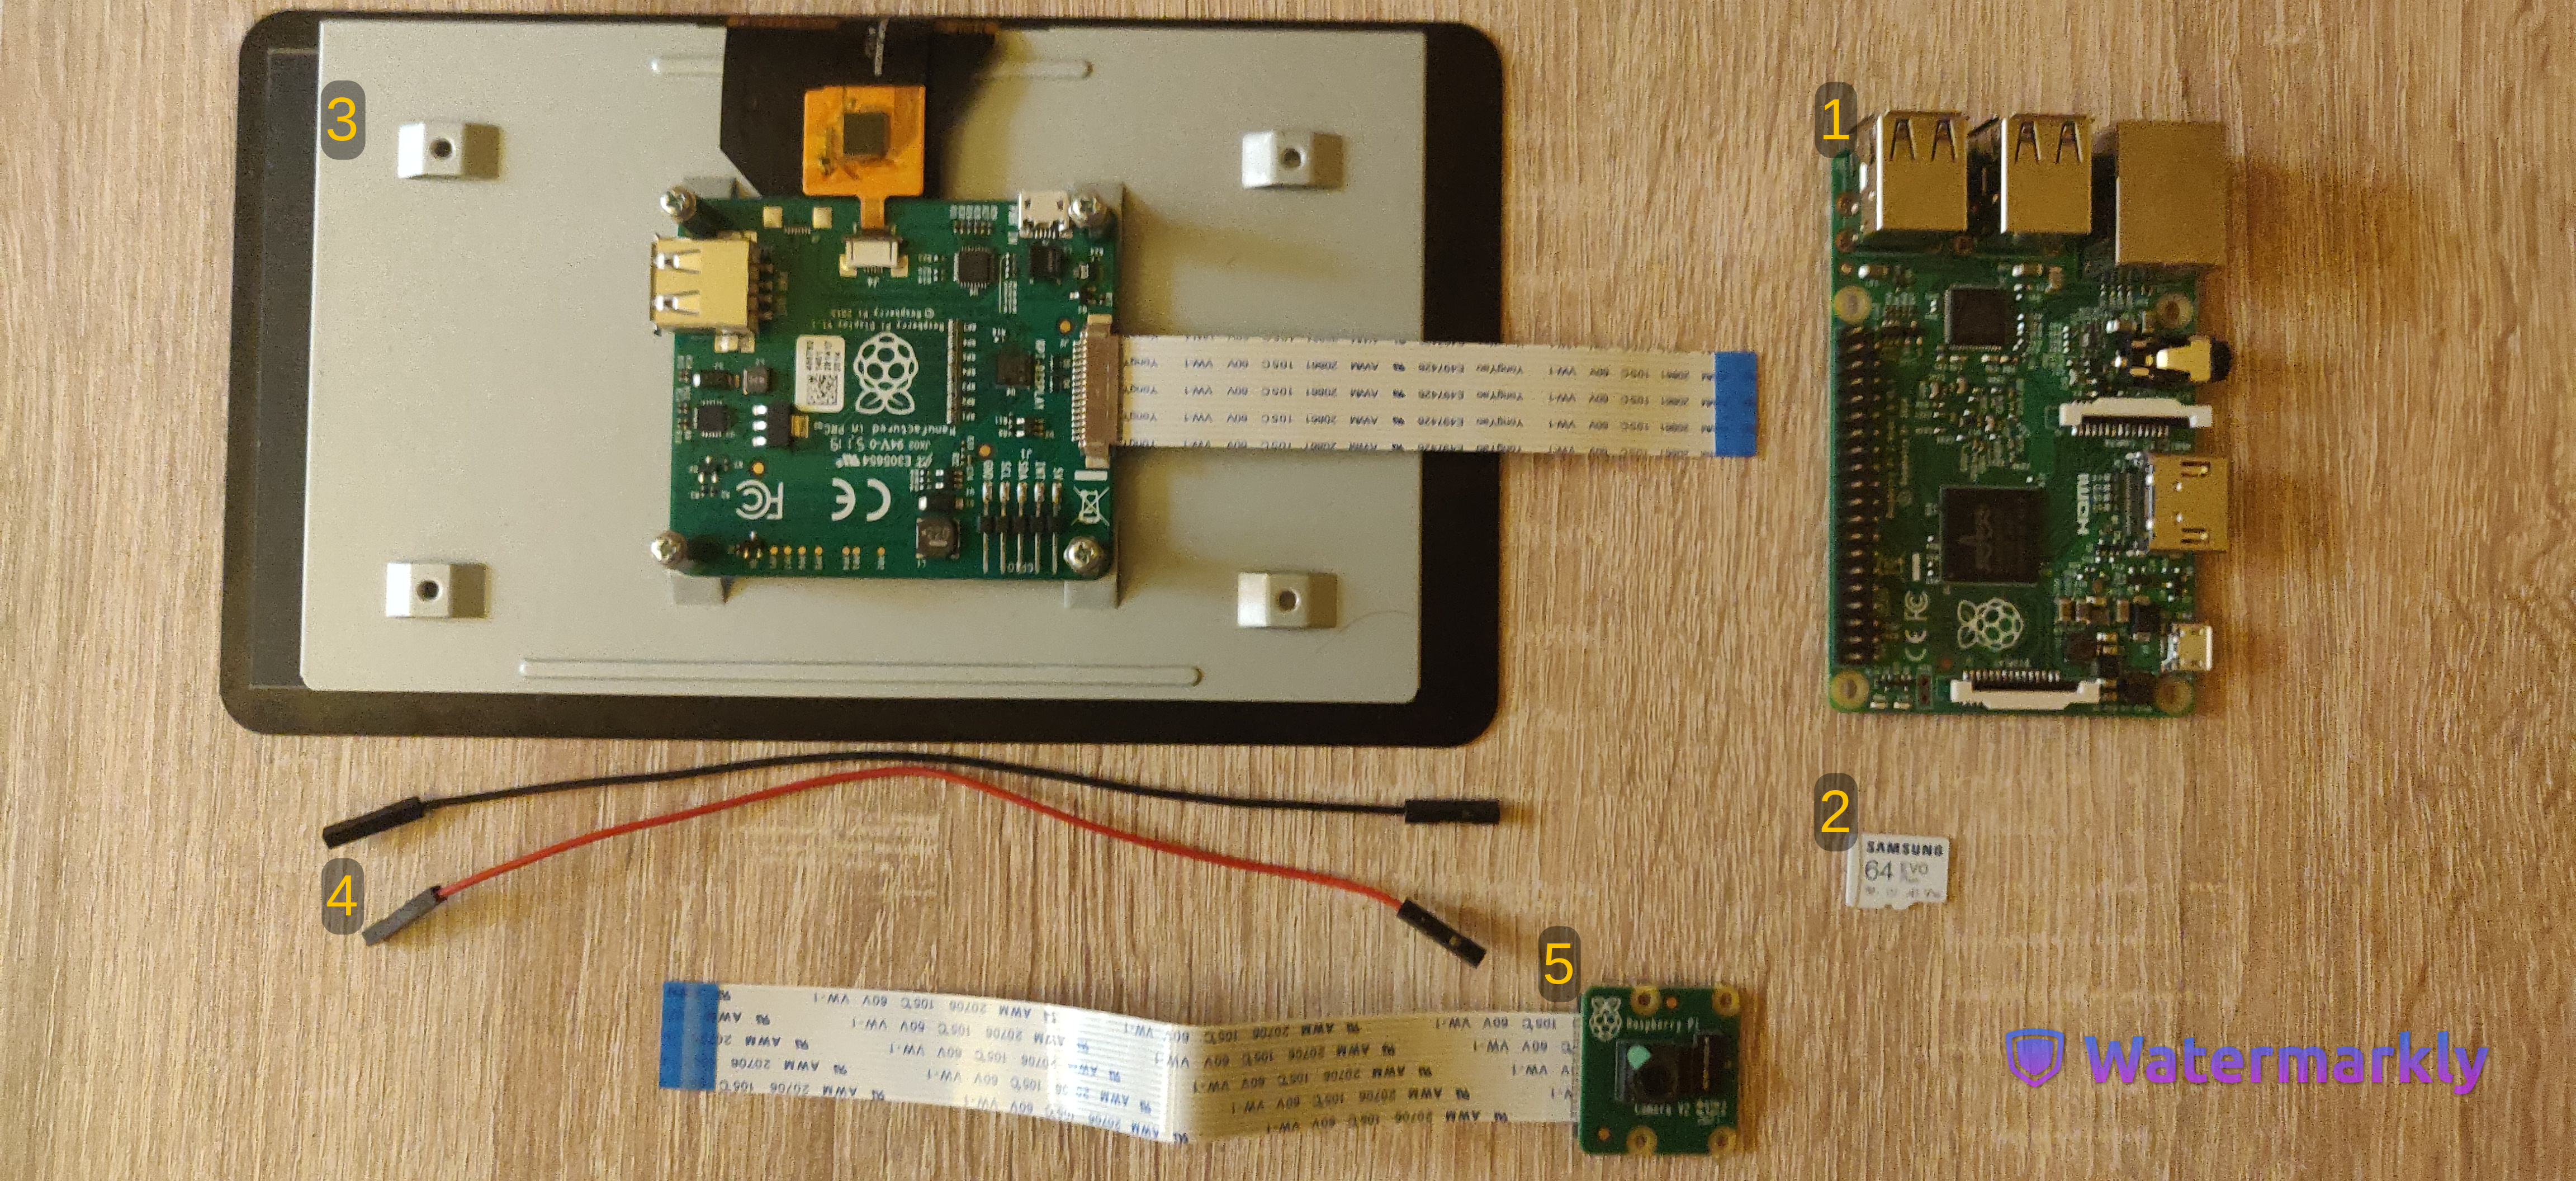
\includegraphics[width=0.95\textwidth, height=0.5\textwidth]{resources/Manual_Components.jpg}
	\caption{Required components}
\end{figure}

Those components are, in order:
\begin{itemize}
	\item 1. Raspberry Pi development board.
	\item 2. SD card for storing operating system.
	\item 3. Raspberry Pi Display, with ribbon cable attached.
	\item 4. Jumper cables for powering display.
	\item 5. Raspberry Pi Camera Module, with ribbon cable attached.
\end{itemize}

Before proceeding with connecting the components, make sure a valid Debian-based operating system is installed
on the SD card. This can be achieved using the methods described within the Raspberry Pi documentation:
\url{https://www.raspberrypi.com/documentation/computers/getting-started.html#installing-the-operating-system}.

The following highlighted ports are used to connect the display and the camera:

\begin{figure}[H]
	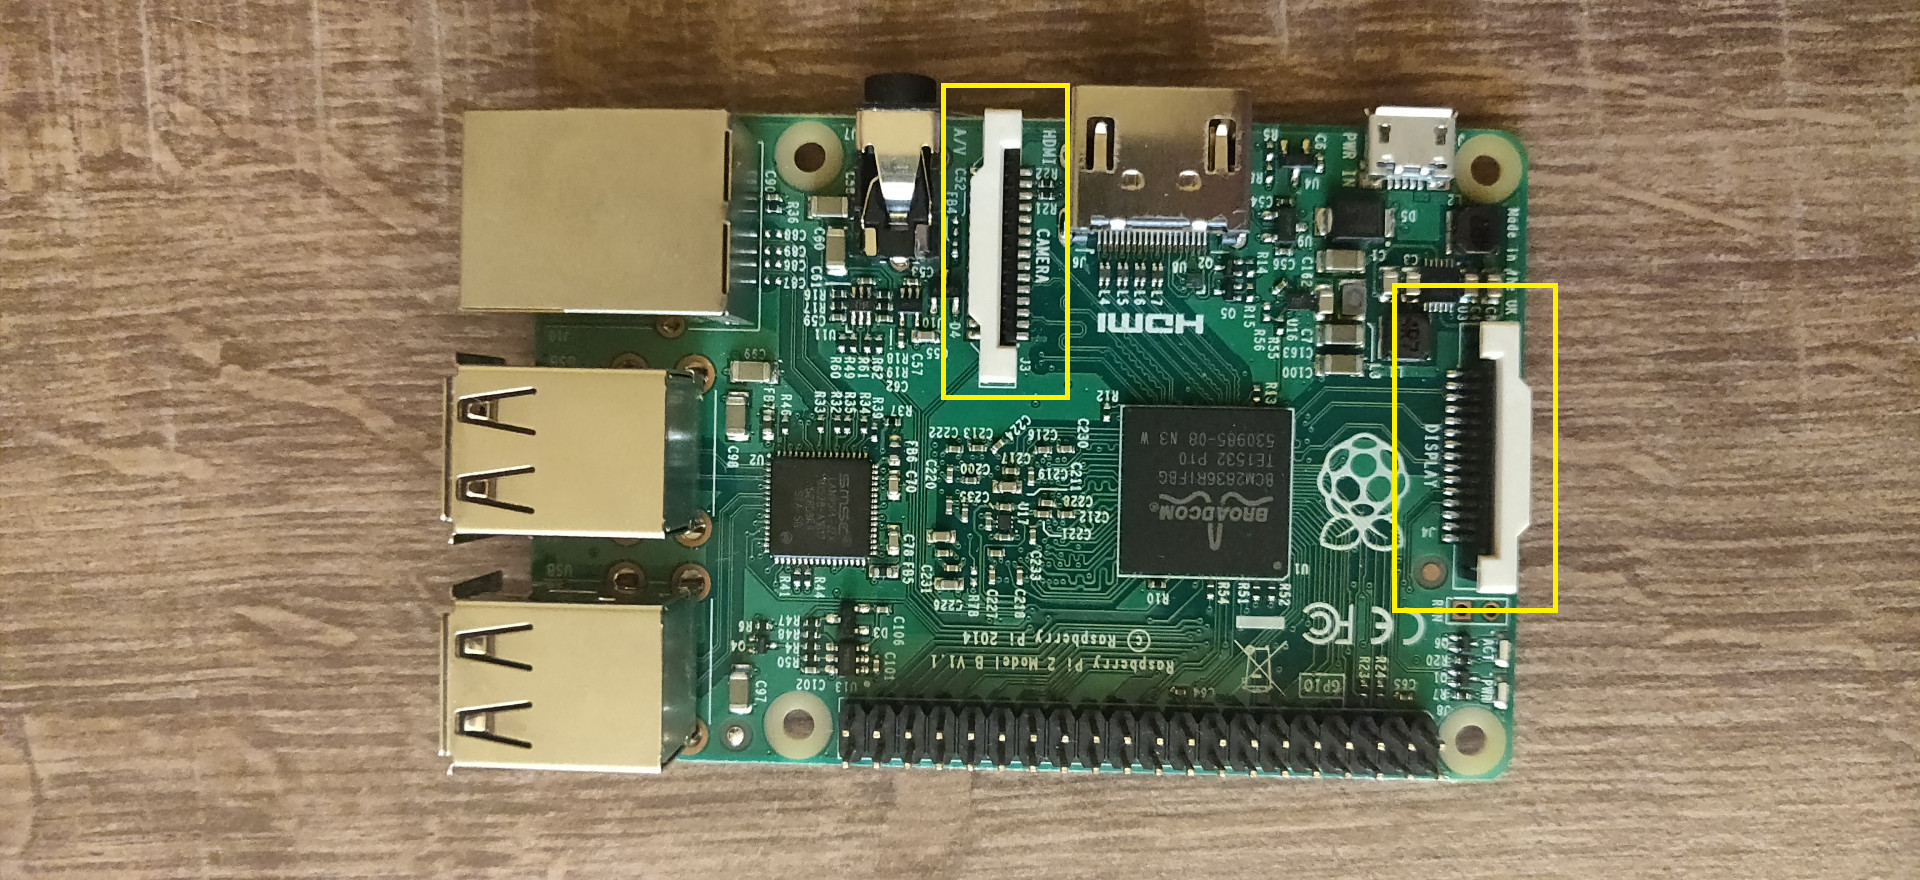
\includegraphics[width=0.95\textwidth, height=0.45\textwidth]{resources/Manual_Connections.jpg}
	\caption{Display and camera connections}
\end{figure}

When making the connection, make sure the pins on the ribbon cable match the pins on the port. Additionally,
the \(5V\) and \(GND\) pins on the display need to be connected to pins \(4\) and \(6\) respectively, on the Raspberry Pi.
Please refer to \url{https://www.raspberrypi.com/documentation/computers/raspberry-pi.html} in order to assess
the boards GPIO pinout.

\begin{figure}[H]
	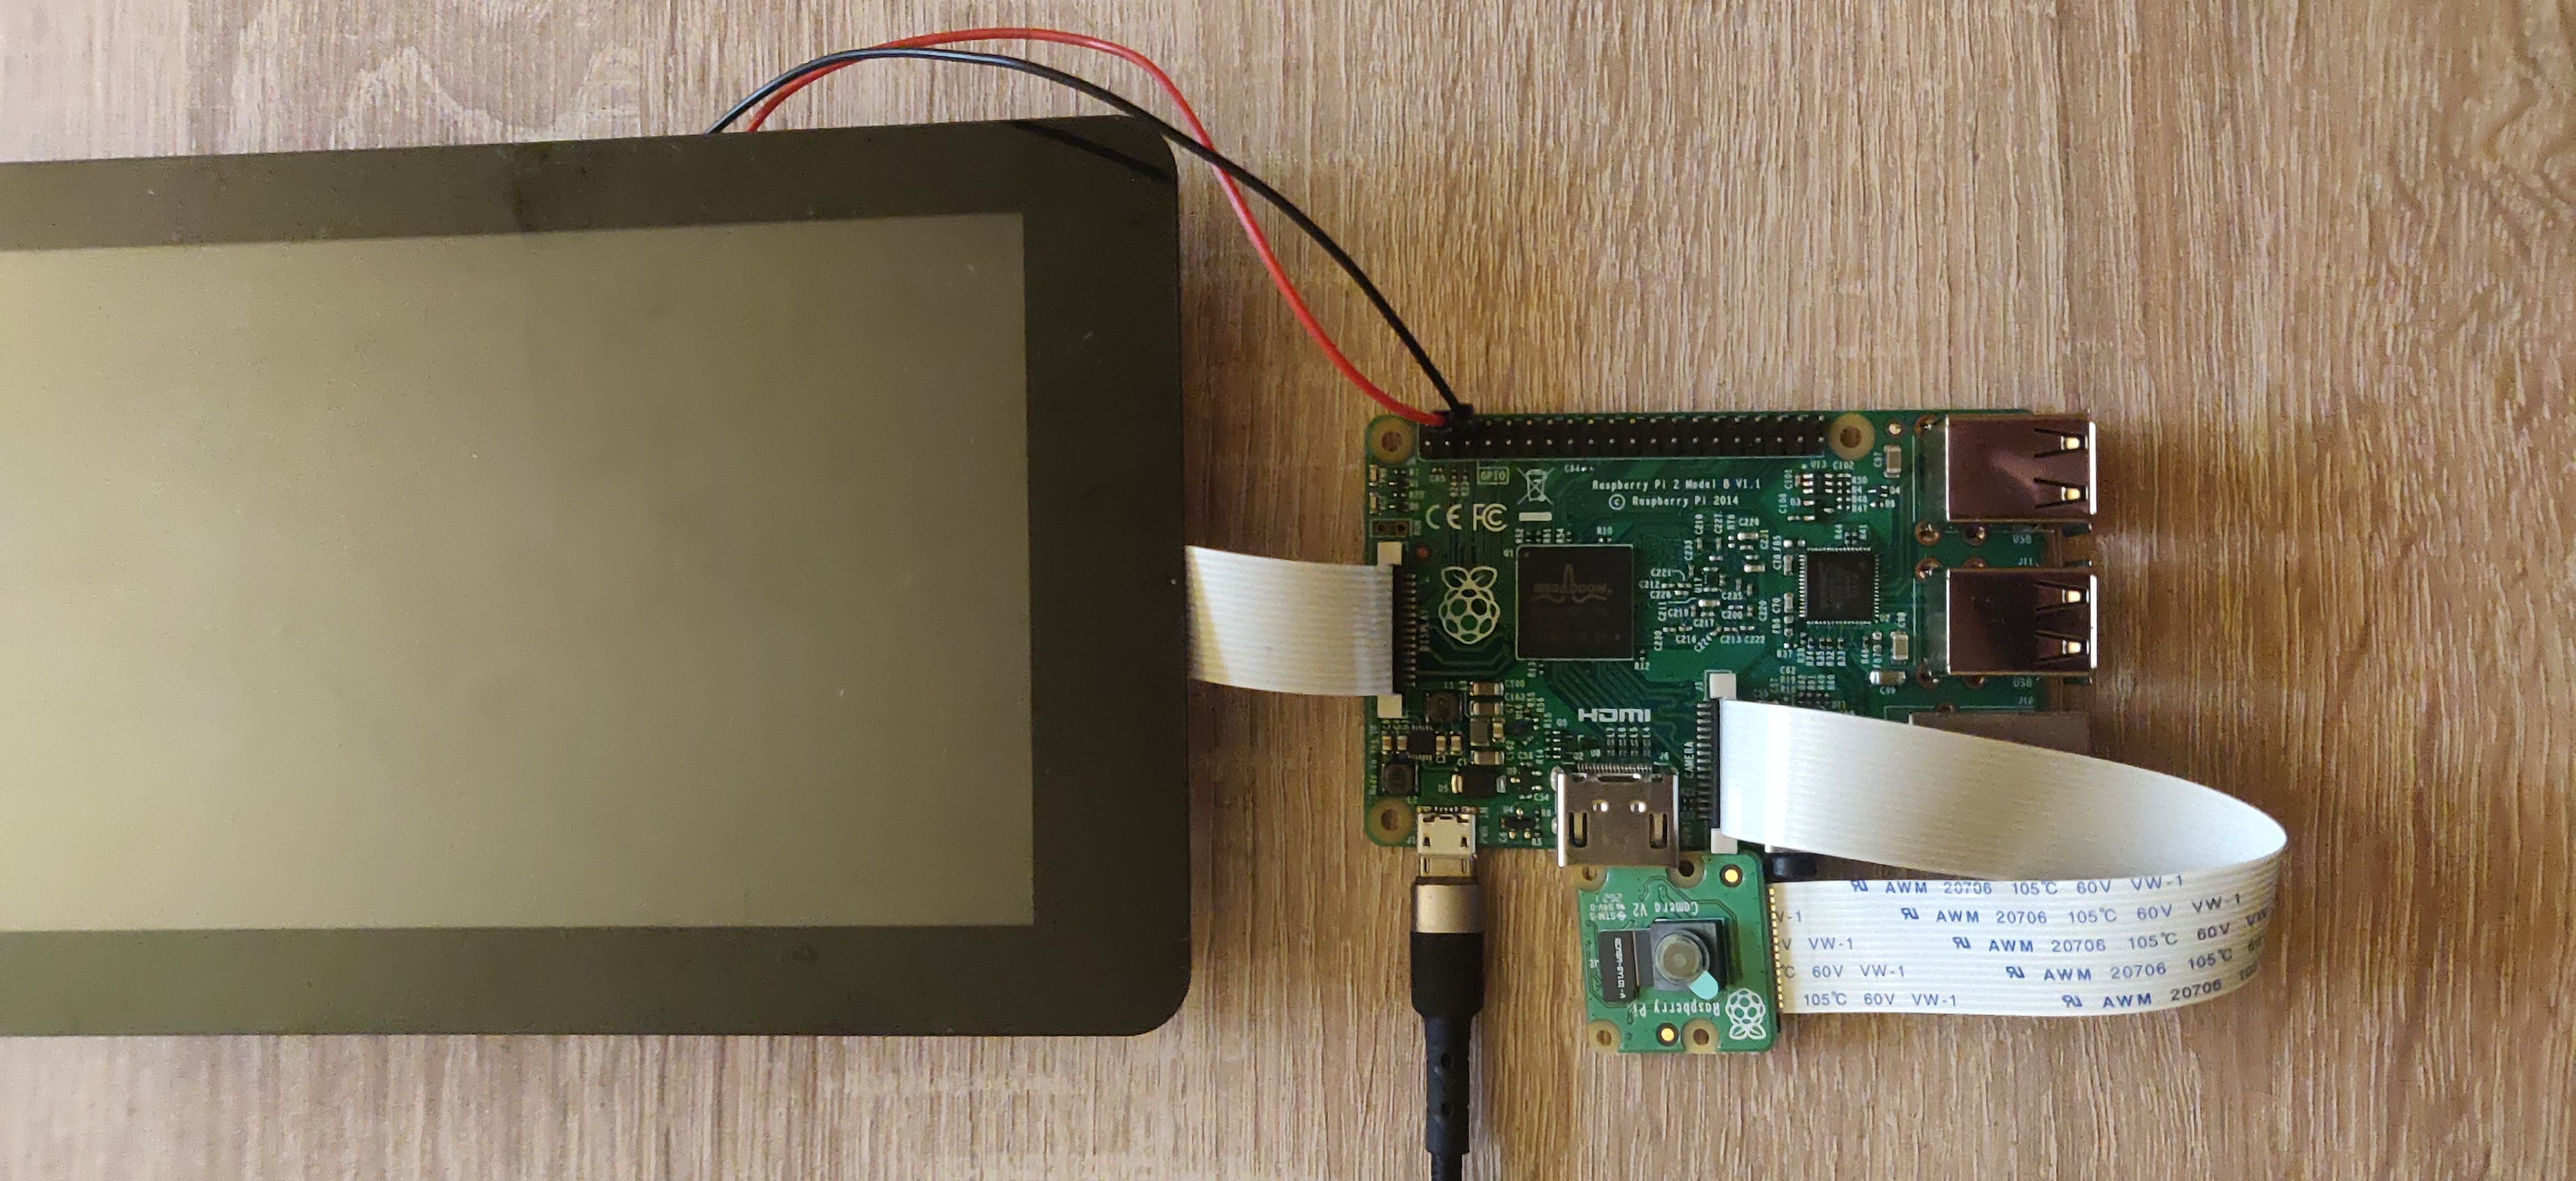
\includegraphics[width=0.95\textwidth, height=0.45\textwidth]{resources/Manual_Setup.jpg}
	\caption{Final setup}
\end{figure}

After all connections are made, the Raspberry Pi can be plugged in. The camera and display need to be enabled
using either the \verb|Preferences| menu or the \verb|raspi-config| utility, depending on the operating system.
An example can be consulted at the following address:
\url{https://techoverflow.net/2019/07/23/how-to-enable-raspberry-pi-camera-using-raspi-config/}.

Additionally, the board can be secured to the display, in order to help with the safety and portability of the
entire setup.

\section{Installation}

After installing \verb|git| or \verb|zip| on the system, copy the source code from
\url{https://github.com/VToporan/ISP_Demo/}

Navigate to the source directory and use the \verb|dependencies.sh| script as superuser, in order to install
all required dependencies, or install them manually, using the systems package manager:
\begin{code}
	\begin{lstlisting}
    cd ISP_Demo
    ./dependencies.sh
    \end{lstlisting}
\end{code}
or
\begin{code}
	\begin{lstlisting}
    sudo apt-get install g++
    sudo apt-get install cmake
    sudo apt-get install qt5-default
    sudo apt-get install libopencv-dev
    \end{lstlisting}
\end{code}

After that, use the \verb|install.sh| script in order to build the executable and create a desktop shortcut.
Upon completion, navigate to the desktop and run the application.

\pagebreak
\section{Interface}

Opening the application, the following user interface will be shown:
\begin{figure}[H]
	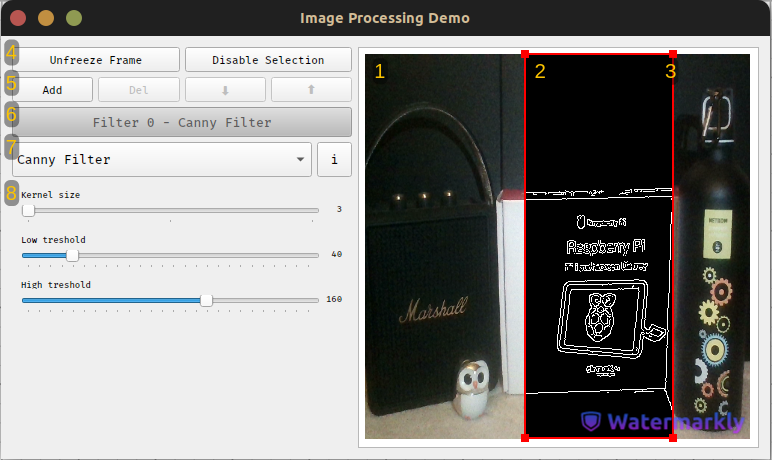
\includegraphics[width=0.95\textwidth, height=0.5\textwidth]{resources/Manual_Outline.jpg}
	\caption{User Interface Overview}
\end{figure}

It can be separated into the following subsections:
\begin{itemize}
	\item 1. Viewport - the resulting image, after all filters are applied, will be shown here.
	\item 2. Region of interest - any given filter will be applied only within its designated ROI.
	\item 3. ROI anchors - used to resize the region of interest.
	\item 4. Miscellaneous - used to pause the frame capture and disable the ROI selection.
	\item 5. Filter management - used to add, delete or change a filters application order.
	\item 6. Filter showcase - used to chose the active ROI and preview filter application order.
	\item 7. Filter selection - used to change the currently applied filter, as well as provide
	      information about parameters.
	\item 8. Parameter management - used to tweak filter parameters in order to change resulting image.
\end{itemize}

\addtocontents{toc}{\protect\setcounter{tocdepth}{5}}



